\documentclass{article}
\usepackage{graphicx}

\usepackage{amssymb}
\usepackage{mathtools}
\usepackage{blindtext}
\usepackage{caption}
\usepackage[a4paper]{geometry}
\geometry{top=2.5cm, bottom=2.5cm, left=2.5cm, right=2.5cm}
\usepackage{fancyhdr}
\pagestyle{fancy}
\usepackage{hyperref}
\hypersetup{colorlinks=true,urlcolor=blue}
\usepackage{wrapfig}

\fancyhead[LO,RE]{Mètodes numèrics II}
\fancyhead[RO,LE]{PRÀCTICA 1}

\graphicspath{ {images/} }

\begin{document}
\thispagestyle{empty}
\begin{center}
    {\LARGE \textsc{Pràctica 1: Modelització del tractament}}\\ 
    \vspace{0.2cm}
    {\LARGE \textsc{d'abalció cardíaca IVS}}\\ 
    \vspace{0.2cm}
    $\begin{matrix} 
    \text{Miguel A.} \hspace{1.5cm} & \text{Daniel G.} & \hspace{1.5cm} \text{Gerard B.}\\1637738 \hspace{1.5cm} & 1666471 & \hspace{1.5cm} 1670235
    \end{matrix}$
\end{center}
\section{Introducció i problema}
Una ablació cardíaca IVS és una cirugia simple que s'aplica a pacients que pateixen arritmies i que reaccionen negativament a tractaments amb fàrmacs. De forma simplificada, aquesta intervenció consisteix en introduïr electrodes de polaritat oposada i local·litzar-los al cor sobre el teixit malalt. L'objectiu és fer servir l'efecte Joule per a escalfar el teixit malalt i provocar-ne la mort cel·lular de forma local. A l'hora d'aplicar aquest procediment quirúrgic cal tenir en compte algunes precaucions. La regió de teixit malalt ha d'estar entre els \(50\,\text{ºC}\) i \(80\,\text{ºC}\), la regió sana no ha de superar els \(50\,\text{ºC}\) i cap regió ha de sobrepassar els \(80\,\text{ºC}\).\\\\
A aquesta pràctica intentarem modelitzar aquest procediment realitzant diferents aproximacions i tenint en compte algunes restriccions. Trobarem una solució analítica al problema i la commpararem amb diverses solucions numèriques simulades amb Fortran.\\\\
Per a modelitzar el problema farem servir la llei de Fourier per a la temperatura:
\begin{equation*}
    c_{v}\rho \frac{\partial T}{\partial t} = \nabla (\kappa \nabla T) + P_{\text{ext}}
\end{equation*}
on $c_{v}$ és la calor específica, $\rho$ és la densitat, $\kappa$ és la conductivitat tèrmica i $P_{\text{ext}}$ fa referència a totes les fonts de calor externes del sistema. El model simplificat que farem servir serà in condensador planoparal·lel format per dos superfícies circulars que defineixen un volum cilíndric on hi ha teixit sa i teixit malalt al centre. Per aplicar més simplificacions al problema, asumirem que aquest teixit malalt també ocupa un volum cilíndric (veure Figura \ref{esquema_model}). 

\begin{figure}[h]
    \centering
    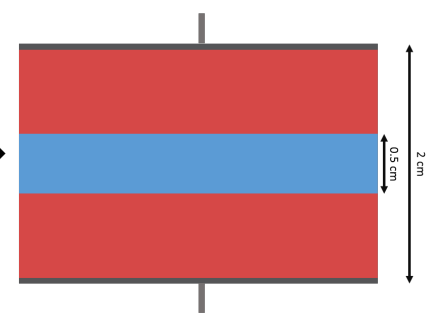
\includegraphics[width = 0.4\linewidth]{images/esquema_temp.png}
\end{figure}

Com a condicions inicials i de frontera tindrem en compte la temperatura del cos humà: \(T_c = 36.5\,\text{ºC}\). Aquesta temperatura ha de manternir-se sempre constant ja que el flux de sang provinent de la resta del cos no para en cap moment.
\section{Equació problema i adimensionalització}
A partir de la llei de d'Ohm podem trobar l'aportació externa de calor obtinguda per efecte Joule:
\begin{equation*}
    \vec{J} = \sigma\vec{E} \hspace{0.3cm} \Rightarrow \hspace{0.3cm} P_{\text{ext}} = \vec{J}\cdot\vec{E} = \sigma E^2 = \frac{\sigma}{2} \frac{(\Delta \phi)^2}{D^2}
\end{equation*}
on $\sigma$ és la conductivitat elèctrica del teixit i $D$ i $\Delta \phi$ son la distància i la diferència de potencial elèctric entre els electrodes, respectivament. Aprofitant la simetria cilíndrica del model, podem escriure la llei de Fourier com
\begin{equation*}
    c_{v}\rho \frac{\partial T}{\partial t} = \kappa \frac{\partial ^2 T}{\partial z^2} + \frac{\sigma}{2} \frac{(\Delta \phi)^2}{D^2}
\end{equation*}
A partir de definir
\begin{equation*}
    T = aT' \hspace{0.3cm} \text{,} \hspace{0.3cm} t = bt' \hspace{0.3cm} \text{,} \hspace{0.3cm} z = cz'
\end{equation*}
Trobem l'equació normalitzada que farem servir per a resoldre el nostre problema:
\begin{equation*}\label{EDP_norm}
    \frac{\partial T'}{\partial t'} = \frac{\partial ^2 T'}{\partial z'^2} + 1 
\end{equation*}
\section{Solució analítica de la EDP}
Com hem dit, els següents apartats els dedicarem a resoldre l'equació diferencial en derivades parcials \eqref{EDP_norm}. Notem que aquesta equació té solució analítica. Al resoldre l'equació seguint el procediment que s'observa a l'Annex \ref{Annex I} obtenim la següent solució normalitzada:
\begin{equation*}
    T'(x,t) = T_c' + \sum_{i=0}^{\infty} \frac{ 1-e^{-(2n+1)^2 pi^2 t}}{(2n+1)^3\pi^3}\cdot 4sin((2n+1)\pi x)
\end{equation*}


\section{Solució numèrica: Euler Explícit}
Fem servir el mètode d'Euler Explícit amb diversos mallats per trobar la distribució de temperatures en $t=0.025$. En la Taula 1, s'exposa el resultat amb el mallat 0,51 i es pot observar com la solució oscil·la en forma de "dents de serra". Això és la inestabilitat numèrica degut a la ximplesa del mètode i fer servir un pas temporal massa gran.  En la Taula 2 i 3 s'exposa el resultat pel mallat de 0,49 i 0,25. Notem que per mallats menors a 0,5 desapareixen les fluctuacions i la solució de l'equació de difusió es fa estable.


\begin{table}[h]
    \centering
    \caption{Resultats pel mallat de 0.51 amb Euler Explícit}
    \label{tab:euler_at1}
    \begin{tabular}{cc}
        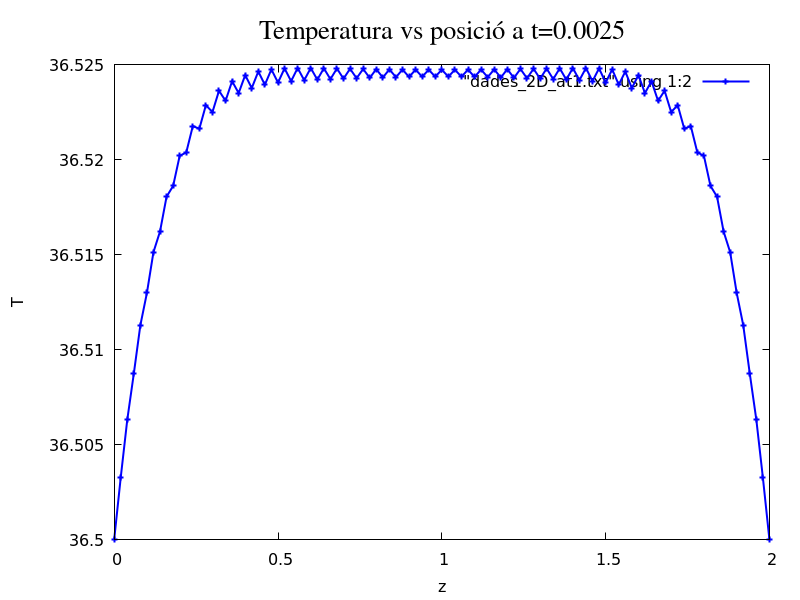
\includegraphics[width=0.4\textwidth]{images/T_vs_z_at1.png} &
        \includegraphics[width=0.4\textwidth]{imagen2.jpg} \\
        
        \parbox{0.4\textwidth}{\centering Solució pel mallat 0.51 en t=0.025 fent servir el mètode d'euler} &
        \parbox{0.4\textwidth}{\centering Error numèric (respecte a la solució analítica) pel mallat 0.51 en t=0.025 fent servir el mètode d'euler} \\
 
    \end{tabular}
\end{table}
\begin{table}[h]
    \centering
    \caption{Resultats pel mallat de 0.49 amb Euler Explícit}
    \label{tab:euler_at1}
    \begin{tabular}{cc}
        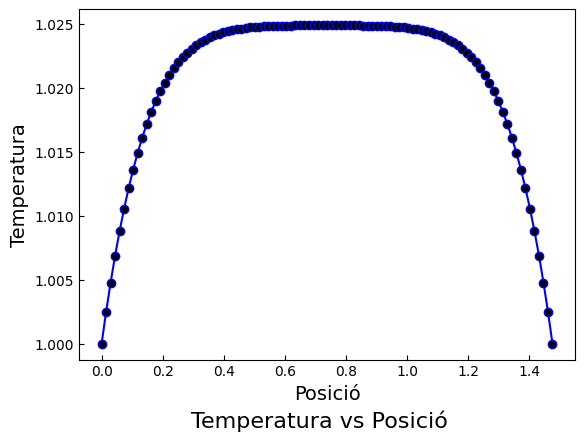
\includegraphics[width=0.4\textwidth]{images/T_vs_z_at2.png} &
        \includegraphics[width=0.4\textwidth]{imagen2.jpg} \\
        
        \parbox{0.4\textwidth}{\centering Solució pel mallat 0.49 en t=0.025 fent servir el mètode d'euler} &
        \parbox{0.4\textwidth}{\centering Error numèric (respecte a la solució analítica) pel mallat 0.49 en t=0.025 fent servir el mètode d'euler} \\
 
    \end{tabular}
\end{table}
\begin{table}[h]
    \centering
    \caption{Resultats pel mallat de 0.51 amb Euler Explícit}
    \label{tab:euler_at1}
    \begin{tabular}{cc}
        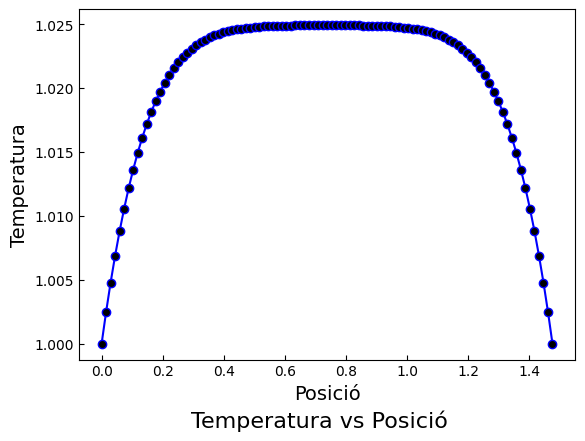
\includegraphics[width=0.4\textwidth]{images/T_vs_z_at3.png} &
        \includegraphics[width=0.4\textwidth]{imagen2.jpg} \\
        
        \parbox{0.4\textwidth}{\centering Solució pel mallat 0.25 en t=0.025 fent servir el mètode d'euler} &
        \parbox{0.4\textwidth}{\centering Error numèric (respecte a la solució anakítica) pel mallat 0.25 en t=0.025 fent servir el mètode d'euler} \\
 
    \end{tabular}
\end{table}

\section{Solució numèrica: Euler Implícit}
\section{Solució numèrica: Crank-Nicolson}
\section{Comparació entre solucions}

\section{Solució del problema d'IVS}
Per determinar el temps necessari hem d'aplicar la senyal elèctrica per tractar eficientment al pacient, farem servir Crank-Nicolson per solucionar l'equació de difusió. Amb aquest mètode, anem trobant iterativament la distribució de temperatura per a un temps creixent. En cada iteració avaluem les temperatures cercant el tractament més eficient possible. Per aconseguir això, a cada distribució de temperatura per una mateixa posició temporal imposem diverses condicions. \\ Primerament que en cap posició espacial pel temps t s'arribi a una temperatura superior o igual a 80ºC. Segonament, que cap part de la regió sana (per $x\in(0,0.75) \cup (1.25,2)$ en cm) arribi o superi els 50ºC. Imposant aquestes dues condicions iterativament arribem a un temps màxim en el qual es compleixen. Amb aquest temps, ens assegurem que per aquest i temps menors el tractament no serà perillós pel pacient. Ara, cerquem que la màxima regió de teixit malalt estigui entre 50ºC i 80ºC. Com hem imposat que en la frontera entre teixits ($x =0.75cm$ i $x=1.25cm$) s'arribes a la temperatura màxima però inferior a 50ºC, tot el teixit malalt es trobara a una temperatura superior. Llavors, la regió més externa del teixit malalt arriba com a mínim a 50ºC en el temps màxim que hem trobat. Això es pot comprovar en la figura \ref{fig:solucion_ivs}, on en vermell es mostra la frontera entre el teixit malalt i el saludable. La figura mostra la distribució de la temperatura pel temps $t =  63.17$ que es la nostra proposta com a temps més eficient i que compleix les condicions imposades. Entre les franjes vermelles es troba el teixit malalt, que podem comprovar que es trobara per damunt de 50ºC, i per fora de les franjes s'observa el teixit saludable que no supera els 50ºC.

\begin{figure}[h]
    \centering
    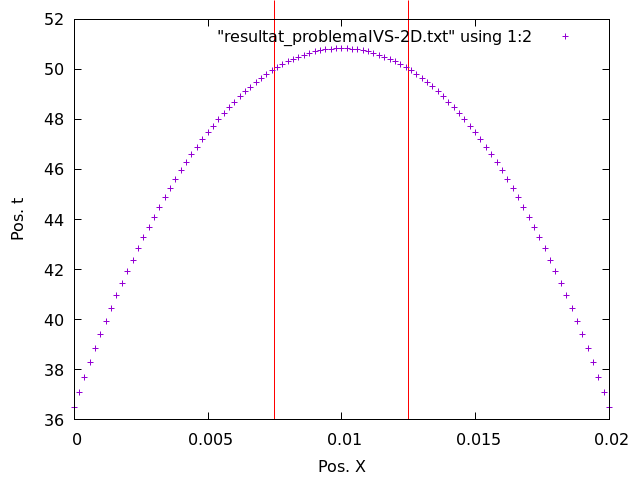
\includegraphics[width=0.5\linewidth]{images/solucion_IVS-2D.png}
    \caption{Distribució de temperatura per al temps màxim trobat de 63.17 segons}
    \label{fig:solucion_ivs}
\end{figure}

\section{Conclusions}
En esta práctica, hemos modelado el proceso de ablación cardíaca IVS para evaluar su eficacia y %
seguridad utilizando diferentes métodos numéricos. A partir de la solución analítica de la ecuación de difusión de calor y las simulaciones numéricas implementadas con métodos explícitos, implícitos y de Crank-Nicolson, se logró determinar el tiempo óptimo de aplicación del tratamiento eléctrico que satisface las condiciones de seguridad requeridas: mantener el tejido sano por debajo de los 50 ºC, evitar que cualquier punto alcance los 80 ºC, y asegurar que la mayor parte del tejido enfermo permanezca entre los 50 ºC y los 80 ºC.

Los resultados numéricos muestran que el método de Crank-Nicolson ofrece un equilibrio óptimo entre precisión y estabilidad, superando las limitaciones de los métodos explícito e implícito en cuanto a oscilaciones o sobrecostos computacionales. De este modo, se determinó que el tiempo ideal para este procedimiento es de 192.78 segundos, garantizando un tratamiento eficiente y seguro.

Finalmente, esta práctica demuestra la utilidad de las técnicas de modelado y simulación numérica en contextos médicos, brindando herramientas para mejorar la comprensión y la implementación de procedimientos clínicos.

\section{Annex}\label{Annex I}
\subsection{Solució analítica}
Sigui una equació del tipus
\begin{equation*}
    \dot{f} = f'' + q
\end{equation*}
on $f = f(x,t)$, $q =q(x,t)$ i on el punt representa derivada parcial temporal i les primes derivades parcials erspecte a $x$.
\end{document}